\documentclass{article}

% if you need to pass options to natbib, use, e.g.:
%     \PassOptionsToPackage{numbers, compress}{natbib}
% before loading neurips_2019

% ready for submission
% \usepackage{neurips_2019}

% to compile a preprint version, e.g., for submission to arXiv, add add the
% [preprint] option:
%     \usepackage[preprint]{neurips_2019}

% to compile a camera-ready version, add the [final] option, e.g.:
\usepackage[final]{neurips_2019}

% to avoid loading the natbib package, add option nonatbib:
%     \usepackage[nonatbib]{neurips_2019}

\usepackage[utf8]{inputenc} % allow utf-8 input
\usepackage[T1]{fontenc}    % use 8-bit T1 fonts
\usepackage{hyperref}       % hyperlinks
\usepackage{url}            % simple URL typesetting
\usepackage{booktabs}       % professional-quality tables
\usepackage{amsfonts}       % blackboard math symbols
\usepackage{nicefrac}       % compact symbols for 1/2, etc.
\usepackage{microtype}      % microtypography

\usepackage{algorithm}
\usepackage{algorithmic}
\usepackage{graphicx}
\usepackage{caption}
\usepackage{subcaption}

\title{Bayesian Machine Learning Project - Bayesian nonparametric models for ranked data}

% The \author macro works with any number of authors. There are two commands
% used to separate the names and addresses of multiple authors: \And and \AND.
%
% Using \And between authors leaves it to LaTeX to determine where to break the
% lines. Using \AND forces a line break at that point. So, if LaTeX puts 3 of 4
% authors names on the first line, and the last on the second line, try using
% \AND instead of \And before the third author name.

\author{%
  Armand Gissler\\
  MVA, Departement of Mathematics\\
  ENS Paris-Saclay\\
  61 Avenue du président Wilson, Cachan \\
  \texttt{armand.gissler@ens-paris-saclay.fr} \\
  % examples of more authors
  \And
  Raymond Zhang\\
  MVA, Departement of Mathematics\\
  ENS Paris-Saclay\\
  61 Avenue du président Wilson, Cachan \\
  \texttt{raymond.zhang@ens-paris-saclay.fr} \\
  % \texttt{email} \\
  % \AND
  % Coauthor \\
  % Affiliation \\
  % Address \\
  % \texttt{email} \\
  % \And
  % Coauthor \\
  % Affiliation \\
  % Address \\
  % \texttt{email} \\
  % \And
  % Coauthor \\
  % Affiliation \\
  % Address \\
  % \texttt{email} \\
}

\begin{document}

\maketitle

\begin{abstract}
  This document is mostly based on the work of Caron and Teh \cite{caron_bayesian_nodate,caron_bayesian_nodate-supmat}. We study here the Plackett-Luce choice model. Its goal is to estimate the desirability of items $k$, by looking on different top-$m$ lists. The two versions that we present here allow us to estimate these weights on a static way or a dynamic way (i.e depending on time). We apply these methods on the African vote for the golden ball trophy 2019 and on the rankings of movies on box-office during the end of 2019 and the beginning of 2020. 
\end{abstract}

\section{Static Bayesian nonparametric ranking models}
In this part we are going to present the Plackett-Luce model, its Bayesian version and the non parametric extension introduced in the article. We are going to apply it to the African vote for the golden ball trophy 2019.

\subsection{The original Plackett-Luce model}

The Original Plackett-Luce model was introduced in \cite{luce2012individual} to model ordered list of top-$m$ items. Those type of data arise often, for example if you ask people to give their top-$m$ best movies of all time. Throughout this part, let us suppose the data we observe are a finite number of partial rankings of length $m$ indexed by $l \in [L]$. Are present in those rankings $K$ different objects and for each object $k\in [K]$,let $n_k$ be the number of time the object appears.

The finite model assumes that for each item $k \in [M] = \{1,2,...,M\}$, is assigned a positive rating parameter $w_k$, called desirability. 

The model generates a top-$m$  $\rho=(\rho_1,\cdots,\rho_m)$ of items of $[M]$ list the following way.

At each stage $i=1,\cdots,m$, an item is chosen among the items that have not been chosen yet with probability proportional to its desirability. The probability that a list $\rho$ is chosen is then :
\begin{equation}
P(\rho) = \prod_{i=1}^m\frac{w_{\rho_i}}{\left(\sum_{k=1}^M w_k\right) -\left(\sum_{j=1}^{i-1}w_{\rho_j}\right)}
\label{finit_rank}
\end{equation}


\subsection{Bayesian Plackett-Luce model with gamma prior}

There exist another Thurstonian interpretation (that is theoretically important) to generate a ranking $l$. 
For each item $k \in [M]$ a latent variable $z_{lk} \sim \text{Exp}(w_k)$ is generated. We can think $z_{lk}$ as the arrival time of item $k$ in a race. Then the items are ordered by the time of arrival with $\rho_{li}$ the index of the item that arrived in the $i$th position in the ranking $l$.
It can be shown that this way of generating ranking is equivalent to the previous one and yield the same probability (\ref{finit_rank}) for a given ranking. 

This is illustrated by the toy example in the notebook where the probability of a ranking generated by both methods is estimated by a simple Monte-carlo and is compared to the true one. The data and the PSG players' score is given by France football for the first leg of PSG-Dortmund in the Round of 16 of Champions League 2020.

To compute the probabilities distribution, they define another latent variable $Z_{li} \triangleq z_{\rho_{li} -z_{\rho_{li-1} }}$

It can be shown that the joint distribution of $((\rho_l)^{l\in [L]},(Z_{li})_{i \in [m] }^{l \in L}| (w_k)_{k\in[K]}$ follow
\begin{equation}
    P\left( (\rho_l)^{l\in [L]},(Z_{li})_{i \in [M] }^{l \in [L]} ) \vert (w_k)_{k\in[K]} \right) = \prod_{l=1}^L\prod_{i=1}^m w_{\rho_{li}} \exp \left( -Z_{li}\left(\sum_{k=1}^M w_k-\sum_{j=1}^{i-1} w_{\rho_{lj}} \right) \right)
    \label{jointfinit}
\end{equation}
Then by factorization, the posterior $Z_{li}\vert (\rho_l,w) \sim \text{Exp}\left(\sum_{k=1}^M w_k-\sum_{j=1}^{i-1} w_{\rho_{lj}} \right)$

Now if we suppose a prior on $w_k\sim\text{Gamma}\left(\frac{\alpha}{M},\tau\right)$ the posterior distribution is : 

\begin{equation}
w_k\vert (\rho_l),(Z_{li}),(w_{k'})_{k'\neq k} \sim \text{Gamma}\left(\frac{\alpha}{M}+n_k,\tau +\sum_{l=1}^L\sum_{i=1}^m \delta_{lik}Z_{li}\right)
\label{wfinit}
\end{equation}
Usually $tau$ is set to one as we look at the ratio between the $w$. The rankings are invariant to the rescaling of the mass $w$

With $\delta_{l i k}$ the occurrences indicator define by : 

\begin{equation}
\delta_{l i k}\triangleq\left\{\begin{array}{ll}
0 & \text { if } \exists j<i \text { with } Y_{l j}=X_{k}^{*} \\
1 & \text { otherwise }
\end{array}\right.
\label{delta}
\end{equation}

And for items that do not appear in the list observed, we can define $w_* \triangleq \sum_{k|n_k=0}w_k$. $w_*$ represent the sum of the score of all the items that are not yet observed, it is the cumulative mass of all the items not observed. It can also be interpreted as the probability (if normalize) of a new item arriving at the first place of a new ranking. Its distribution follows 

\begin{equation}
w_* \vert (\rho_l),(Z_{li}),(w_k)_{k,n_k>0} \sim \text{Gamma}\left(\alpha,\tau +\sum_{l=1}^L\sum_{i=1}^m Z_{li}\right)
\label{wrestfinit}
\end{equation}

\subsection{Non parametric Bayesian Plackett-Luce model}

Now let's assume we have an infinite pool of items $(X_k)_{k\ge 1}$ with rankings $(w_k)_{k\ge 1}$. As in (\ref{finit_rank}) we can compute the probability of a top m-list.

\begin{equation}
P(X_{\rho_1},...,X_{\rho_m}) = \prod_{i=1}^m\frac{w_{\rho_i}}{\left(\sum_{k=1}^{+\infty} w_k\right) -\left(\sum_{j=1}^{i-1}w_{\rho_j}\right)}
\label{infinit_rank}
\end{equation}

And to formalize this law and to prove the theorems, they define an atomic measure :
$$
G \triangleq \sum_k^{+\infty}w_k\delta_{X_k}
$$
Then by re-normalize G, we have a atomic probability distribution.
The first item from a list $X_{\rho_1}$ is drown according to G. Then the atom is removed. to draw the next one. There exist theory to treat those kind of problem on permutation of random measure. \cite{pitman2006combinatorial}

Then we can compute the joint probability of 
$((\rho_l)^{l\in [L]},(Z_{li})_{i \in [m] }^{l \in L} )$ knowing $(w)$ i.e. $G$ as in $\ref{jointfinit}$

\begin{equation}
    P\left( (\rho_l)^{l\in [L]},(Z_{li})_{i \in [m] }^{l \in [L]} ) \vert G\right) = \prod_{l=1}^L\prod_{i=1}^m w_{\rho_{li}} \exp \left( -Z_{li}\left(\sum_{k=1}^{+\infty} w_k-\sum_{j=1}^{i-1} w_{\rho_{lj}} \right) \right)
    \label{jointinfinit}
\end{equation}

The same goes for the posterior of $Z_li|(\rho_l,w)$:

\begin{equation}
    Z_{li}\vert (\rho_l,w) \sim \text{Exp}\left(\sum_{k=1}^{+\infty} w_k-\sum_{j=1}^{i-1} w_{\rho_{lj}} \right)
    \label{zlateninfinit}
\end{equation}

Then by taking heuristically $M \rightarrow +\infty$ in \ref{wfinit}, this is shown in the appendix of the article. We have 

\begin{equation}
w^*_k\vert (\rho_l),(Z_{li}),(w^*_{k'})_{k'\neq k} \sim \text{Gamma}\left(n_k,\tau +\sum_{l=1}^L\sum_{i=1}^m \delta_{lik}Z_{li}\right)
\label{winfinit}
\end{equation}

The law of the sum of the weight of items that do not appear in our list stays the same.

\subsection{Gibbs sampling}
With the posterior distribution given by the equation (\ref{zlateninfinit}),(\ref{winfinit}),(\ref{wrestfinit}). And a final one if on put a prior $\text{Gamma}(a,b)$ on $\alpha$ with a,b 2 hyper parameters. We have :

\begin{equation}
    \alpha \vert Z_{li} \sim \text{Gamma}\left(a+K , b + \text{log}\left(1 +\frac{\sum_{l=1}^L\sum_{i=1}Z_{li}}{\tau} \right) \right)
 \label{alphaup}  
\end{equation}

We have the following Gibbs updates: 
\begin{itemize}
    \item update $Z_{li}|\text{rest} \sim \text{Exp}\left(w^*_*-\sum_{k}\delta_{lik} w_k \right)$ with (\ref{zlateninfinit})
    \item update $w^*_k\vert \text{rest} \sim \text{Gamma}\left(n_k,\tau +\sum_{l=1}^L\sum_{i=1}^m \delta_{lik}Z_{li}\right)$ with (\ref{winfinit})
    \item update $\alpha \vert \text{rest} \sim \text{Gamma}\left(a+K , b + \text{log}\left(1 +\frac{\sum_{l=1}^L\sum_{i=1}Z_{li}}{\tau} \right) \right)$ with (\ref{alphaup})
    \item update $w^*_* |\text{rest} \sim \text{Gamma}\left(\alpha,\tau +\sum_{l=1}^L\sum_{i=1}^m Z_{li}\right)$ with (\ref{wrestfinit})
\end{itemize}

We have the pseudo code for the Gibbs sampler algorithm \ref{Gibbs_stat}

\begin{algorithm}
\caption{Gibbs Sampler (Static)}
\label{Gibbs_stat}
\begin{algorithmic}
\REQUIRE $L$ top-$m$ $Y_{l}=(Y_{l1},\cdots,Y_{lm})$ Priors $\alpha$, $\beta$, $N_\text{warmup}$,$N_\text{iteration}$.

\STATE \textbf{Initialization}
\STATE $K \leftarrow$ number of discovered item
\STATE $L \leftarrow$ number of rankings
\STATE $m \leftarrow$ length of a ranking
\STATE $\tau \leftarrow 1$
\STATE $n_k \leftarrow$ number of apparition of item $k$
\STATE $\delta_{lik} \leftarrow $as defined in $\ref{delta}$
\STATE $\alpha\leftarrow\text{Gamma}(a+K,b)$.
\STATE $w^*_{k}\leftarrow \text{Gamma}(n_k,\tau)$.
\STATE $w^*_*\leftarrow \text{Gamma}(\alpha,\tau)$.


\STATE

\FOR{$j=1,\cdots,N_\text{warmup}+N_\text{iterations}$}

\STATE \textbf{Update }$Z_{li}$ :
\FOR{$l,i \in [L]*[m]$}
\STATE $Z_{li} \leftarrow \text{Exp}\left(w^*_*-\sum_{k}\delta_{lik} w_k \right)$
\ENDFOR

\STATE \textbf{Update }$w^*_k$
\FOR{$k=1,\cdots,K$}
\STATE $w^*_k \leftarrow \text{Gamma}\left(n_k,\tau +\sum_{l=1}^L\sum_{i=1}^m \delta_{lik}Z_{li}\right)$
\ENDFOR

\STATE \textbf{Update }$\alpha$
\STATE $\alpha \leftarrow \text{Gamma}\left(a+K , b + \text{log}\left(1 +\frac{\sum_{l=1}^L\sum_{i=1}Z_{li}}{\tau} \right) \right)$

\STATE \textbf{Update }$w_*^*$
$w^*_* | \leftarrow \text{Gamma}\left(\alpha,\tau +\sum_{l=1}^L\sum_{i=1}^m Z_{li}\right)$

\ENDFOR
\end{algorithmic}
\end{algorithm}


\subsection{Numerical result}
We applied the Gibbs sampler on data of the African vote for the golden ball. The data is accessible here : \cite{databallon}. The rule for that election is that each country gives its top 5 players (among a pre-selected pool of 30 player which does not verify the assumption of the infinitely many items...). The first player is attributed 6 points, the second 4 points, the third 3 points the fourth 2 points and the last 1 point. The ranking is then computed based on the number of point collected by each player. In the 2019 edition the African continent elected Messi with 187 point in front of Mané with 170. Let see what the algorithm tells us.

We run this algorithm \ref{Gibbs_stat} on the data with the following parameters : 
\begin{itemize}
    \item $\alpha =10 $
    \item $\beta =1$
    \item $N_\text{warmup} = 10000$
    \item $N_\text{iteration} = 10000$
\end{itemize}
The result are presented in fig. \ref{fig:disrib_weight} and \ref{fig:mean_weight} 

\begin{figure}
    \centering
    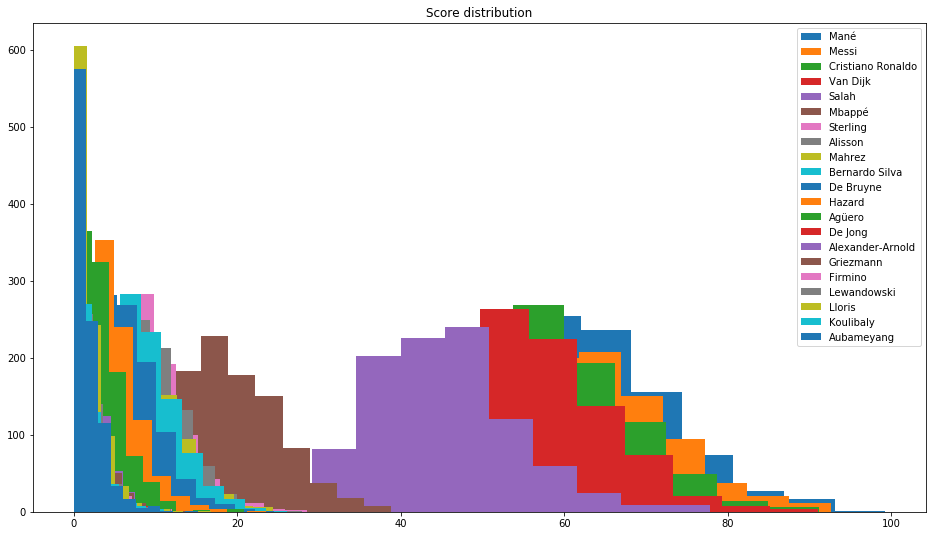
\includegraphics[width = 0.9\textwidth]{Distrib_player.png}
    \caption{Distribution of weights for each player}
    \label{fig:disrib_weight}
\end{figure}

\begin{figure}
    \centering
    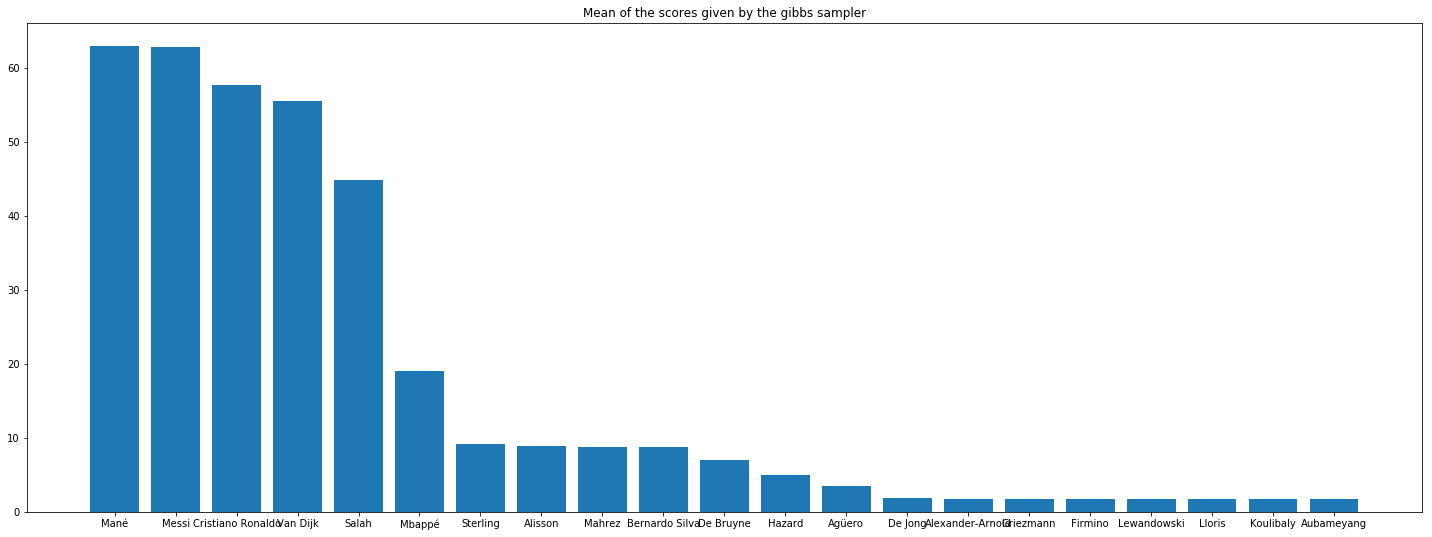
\includegraphics[width = 0.9\textwidth]{mean_score_player.png}
    \caption{Mean of the distribution for each player ranked}
    \label{fig:mean_weight}
\end{figure}
We can add that we have a $w^*_* = 85 $ that $21$ out of $30$ player appeared in the rankings.

We can remark that the model gives Mané first before Messi but are still very close. What may seem strange is that $w^*_*$ is very high compared to the the score of Mane for example. If we draw a top 5 ranking for example by asking the top 5 players from a African journalist, I am not sure that he will put a new a player on top of the his list with this high probability. This is very unintuitive. Maybe this is due to the fact that the pool of player is not infinite (Which I think won't change a lot of thing as the top-5 of many country will stay the same). Or maybe this model is not very suited to the golden ball vote as each ranking is given a different country and each country may have different preferences.
Another hypothesis is that we do not have enough ranking data. 


\newpage

\section{Dynamic Bayesian nonparametric ranking models}

\subsection{Pitt-Walker dependence model}

Suppose $G_t\sim\Gamma(\alpha,\tau,H)$ is a Gamma process. Then, we can write $G_t$ under the following form :
\[
G_t = \sum_{k=1}^\infty w_{tk}\delta_{X_{tk}}
\]
Let us define the random measure $C_t$ conditionnally to $G_t$ :
\[
C_t\vert G_t = \sum_{k=1}^\infty c_{tk}\delta_{X_{tk}} ~~\text{ where } ~~ c_{tk}\vert G_t\sim\text{Poisson}\left(\phi_tw_{tk}\right)
\]
Then, the law of $G_t$ given $C_t$ is given by :
\[
G_t = G_t^*+\sum_{k=1}^\infty w_{tk}^*\delta_{X_{tk}}
\]
where $G_t^*$ and $(w_{tk}^*)_k$ are mutually independents and :
\[
G_t^*\vert C_t\sim\Gamma(\alpha,\tau+\phi_t,H) ~~~~~ w_{tk}^* \vert C_t\sim\text{Gamma}(c_{tk},\tau+\phi_t)
\]
Define then $G_{t+1}=G_{t+1}^*+\sum_{k=1}^\infty w_{t+1,k}\delta_{X_{tk}}$, where $G_{t+1}^*\sim\Gamma(c_{tk},\tau+\phi_t)$. Then, for an atome $X$ with mass $w>0$, the probability that it is dead at time $t$ is given by :
\[
\mathbb{P}\left[ G_t(\lbrace X\rbrace)=0 \vert w\right] = \exp(-y_{t\vert 1}w)
\]
where $y_{t\vert t-1}=\phi_{t-1}$ and $y_{t\vert s-1}=\frac{y_{t\vert s}\phi_{s-1}}{\phi_{s-1}+\tau+y_{t\vert s}}$.

\subsection{Posterior characterization and Gibbs sampling}

At each time $t=1,\cdots,T$, suppose that we observe one top-$m$ list $Y_t=(Y_{t1},\cdots,Y_{tm})$.

Let $X^*=(X_k^*)_{k=1,\cdots,K}$ be the set of unique items observed in $Y_1,\cdots,Y_T$.

Let $n_{tk}\in\lbrace 0,1\rbrace$ be the number of times that $X_k^*$ appears at time $t$ in $Y$.

Define finally $\rho_i$ as $Y_t=(X_{\rho_1}^*,\cdots,X_{\rho_m}^*)$.
Let us denote :
\[
\begin{array}{l}
w_{tk}\doteq G_t(\lbrace X_k^*\rbrace) \\
w_t^* \doteq G_t(\mathbb{X}\setminus X^*) \\
c_{tk}\doteq C_t(\lbrace X_k^*\rbrace) \\
c_t^* \doteq C_t(\mathbb{X}\setminus X^*) \\
\forall t, \forall i, Z_{ti}\sim\text{Exp}\left( w_t^*+\sum_{k=1}^Kw_{tk}^*-\sum_{j=1}^{i-1}w_{t\rho_j}\right)
\end{array}
\]

A Gibbs sampler step is as follows :
\begin{itemize}
\item Update $Z_{ti}$.
\item Update $(w_{tk})\vert(Z_{ti},(c_{tk}),(c_t^*)$.
\item Update $(c_{tk}),(c_t^*)$.
\item Update $\alpha, (w_t^*),(c_t^*)$.
\item Update $(\phi_t)$.
\end{itemize}

\subsection{Numerical experiment}

\subsubsection{Gibbs sampler}

We executed the following algorithm :

\begin{algorithm}
\caption{Gibbs Sampler (Dynamic Plackett-Luce model)}
\begin{algorithmic}
\REQUIRE Set of items $X^*=(X_k^*)_{k=1,\cdots,K}$, $L$ top-$m$ lists at each time $t=1,\cdots,T$ : $Y_{tl}=(Y_{tl1},\cdots,Y_{tlm})$.

\STATE \textbf{Initialization}
\STATE $\alpha\leftarrow\text{Gamma}(a,b)$.
\STATE $\phi\leftarrow\phi_\text{init}$.
\STATE $G_t(\mathbb{X})\leftarrow 1$.
\STATE $w_{tk}\leftarrow\frac{1}{K}$.
\STATE $w_{t*}\leftarrow 0$.
\STATE $c_{tk}\leftarrow\text{Poisson}(\phi w_{tk})$.
\STATE $c_{t*}\leftarrow 0$.
\STATE $Z_{til}\leftarrow\text{Exponential}(1-(i-1)/K)$.
\STATE $n_{tk}\leftarrow\sum_{l=0}^L \sum_{i=1}^m \mathbb{1}_{X_k^*=Y_{tli}}$.

\STATE

\FOR{$j=1,\cdots,N_\text{iterations}$}

\STATE \textbf{Update }$G_t(\mathbb{X})$ :
\STATE $G_0(\mathbb{X})\leftarrow\text{Gamma}(\alpha,\tau)$.
\FOR{$t=1,\cdots,T-1$}
\STATE $M_t\leftarrow\text{Poisson}(\phi G_t(\mathbb{X}))$
\STATE $G_{t+1}\leftarrow\text{Gamma}(\alpha +M_t,\tau+\phi)$.
\ENDFOR
\STATE Change $w_{tk}$ and $w_{t*}$, in order to have $G(\mathbb{X})=\sum_{k=1}^K w_{tk} + w_{t*}$.

\STATE

\STATE \textbf{Update }$c_{tk}$
\STATE Define $\tau_k^-$ as $\sup\lbrace t=1,\cdots,T \vert \forall u\leqslant t,n_{uk}=0 \rbrace$.
\STATE Define $\tau_k^+$ as $\inf\lbrace t=1,\cdots,T \vert \forall u\geqslant t,n_{uk}=0 \rbrace$.
\STATE Define $x_T=\sum_{kl}Z_{Tkl}$ and $x_{t}=\sum_{kl}Z_{tkl}+\frac{\phi x_{t+1}}{1+\phi+x_{t+1}}$.
\FOR{$t=\tau_k^-$}
\STATE $c_{tk}\leftarrow\text{Poisson}((1+\phi)/(1+\phi+x_t)\phi w_{tk})$.
\STATE $w_{t+1,k}\leftarrow\text{Gamma}(c_{tk},\tau+\phi+x_t)$.
\ENDFOR

\FOR{$t=\tau_k^-+1,\cdots,\tau_k^+-1$}
\IF{$w_{t+1,k}>0$}
\STATE Propose $\tilde{c}_{tk} = \text{zeroTruncatedPoisson}(\phi w_{tk})$.
\STATE $c_{tk}\leftarrow\tilde{c}_{tk}$ with probability $\frac{\text{Gamma}(w_{t+1,k};\tilde{c}_{tk},\tau+\phi)}{\text{Gamma}(w_{t+1,k};c_{tk},\tau+\phi)}$.
\ELSE
\STATE $c_{tk}\leftarrow 0$ with probability $\frac{1}{1+\phi w_{tk}(\tau+\phi)}$.
\STATE $c_{tk}\leftarrow 1$ otherwise.
\ENDIF

\ENDFOR

\FOR{$t=\tau_k^+$}
\STATE $c_{tk}\leftarrow\text{Poisson}((1+\phi)/(1+\phi+x_t)\phi w_{tk})$.
\STATE $w_{t+1,k}\leftarrow\text{Gamma}(c_{tk},\tau+\phi+x_t)$.
\ENDFOR


\STATE

\STATE \textbf{Update }$\alpha$
\STATE Define $y_T=0$ and $y_{t-1}=y_t-\log \frac{1+\phi}{1+\phi+x_t}$.
\STATE $\alpha\leftarrow\text{Gamma}(a+K,b+y_1+\log(1+x_1))$.

\STATE

\STATE \textbf{Update }$c_{t*}$ \textbf{and} $w_{t*}$
\STATE $w_{1*}\leftarrow\text{Gamma}(\alpha,\tau+x_1)$.
\FOR{$t=1,\cdots,T-1$}
\STATE $c_{t*}\leftarrow\text{Poisson}((1+\phi)/(1+\phi+x_{t+1})\phi w_{t*})$.
\STATE $w_{t+1*}\leftarrow\text{Gamma}(\alpha+c_{t*},\tau+\phi+x_{t+1})$.
\ENDFOR

\STATE
\STATE
\STATE
\STATE
\STATE
\STATE
\STATE
\STATE
\STATE
\ENDFOR
\end{algorithmic}
\end{algorithm}

\begin{algorithm}
\begin{algorithmic}

\FOR{$j=1,\cdots,N_\text{iterations}$}
\STATE \textbf{Update }$w_{tk},w_{t*}$.
\FOR{$t=1,\cdots,T$}
\FOR{$k=1,\cdots,K$}
\IF{$c_{tk}+c_{t-1,k}+n_{tk}=0$}
\STATE $w_{tk}\leftarrow 0$.
\ELSE
\STATE Define $\delta_{tkil}=0$ if $\exists \hat{i}\leqslant i, Y_{tl\hat{i}}=X^*_k$, and $1$ otherwise.
\STATE $w_{tk}\leftarrow\text{Gamma}(n_{tk}+c_{t-1,k}+c_{tk},\tau+2\phi+\sum_{i,l}\delta_{tkil}Z_{til})$.
\ENDIF
\ENDFOR
\STATE $w_{t*}\leftarrow\text{Gamma}(\alpha+c_{t*}+c_{t-1*},\tau+2\phi+\sum_{i,l}Z_{til})$.
\ENDFOR

\STATE

\STATE \textbf{Update }$Z_{til}$
\STATE $Z_{til}\leftarrow\text{Exponential}(1/(w_{t*}+\sum_{k}\delta_{tikl}w_{tk}))$.

\STATE

\STATE \textbf{Update }$\phi$
\STATE Propose $\tilde{\phi}=\phi\exp(\sigma\varepsilon)$, for $\varepsilon\sim\mathcal{N}(0,1)$.
\STATE $\phi\leftarrow\tilde{\phi}$ with probability :
{\small
\begin{align*}
\min \left( 1 , \frac{p(\tilde{\phi})}{p(\phi)}\frac{\phi}{\tilde{\phi}}\prod_{t=1}^{T-1} \exp\right. & \left( w_{t+1,*}\frac{\phi-\tilde{\phi}}{(\tau+\tilde{\phi}+x_t)(\tau+\phi+x_t)}\right)\left(\frac{\tau+\phi+x_t}{\tau+\tilde{\phi}+x_t}\right)^{\alpha+c_{t*}} \\
& \left. \prod_{k:w_{tk}>0} \exp\left( w_{t+1,k}\frac{\phi-\tilde{\phi}}{(\tau+\tilde{\phi}+x_t)(\tau+\phi+x_t)}\right)\left(\frac{\tau+\phi+x_t}{\tau+\tilde{\phi}+x_t}\right)^{\alpha+c_{tk}} \right)
\end{align*}}

\STATE

\IF{$j\geqslant N_\text{iterations}-N_\text{sample}$}
\STATE $w_{t,k}^{(j-N_\text{sample})}\leftarrow w_{t,k}$.
\STATE $w_{t*}^{(j-N_\text{sample})}\leftarrow w_{t*}$.
\ENDIF
\ENDFOR

\RETURN{$w_{t,k}^{(j)},w_{t*}^{(j)}$ for $j=0,\cdots,N_\text{sample}-1$}
\end{algorithmic}
\end{algorithm}
\newpage
\subsubsection{Parameters}

We have used :
\begin{itemize}
\item As a data set, the top-5 box-office movies, each week between October 2019 and February 2020, in US, France, UK and Germany\cite{datamovies}.
\item $a=0.01,b=0.01$.
\item $\phi_\text{init}=10^{-5}$.
\item $\tau=1$.
\item $N_\text{iterations}=10^{5}$, $N_\text{sample}=1/2\times N_\text{iterations}$.
\end{itemize}

\newpage

\subsubsection{Results}

We obtained the following weights $w_{tk}$, after renormalization :


\begin{figure}[h!]
  \begin{subfigure}[b]{0.6\textwidth}
    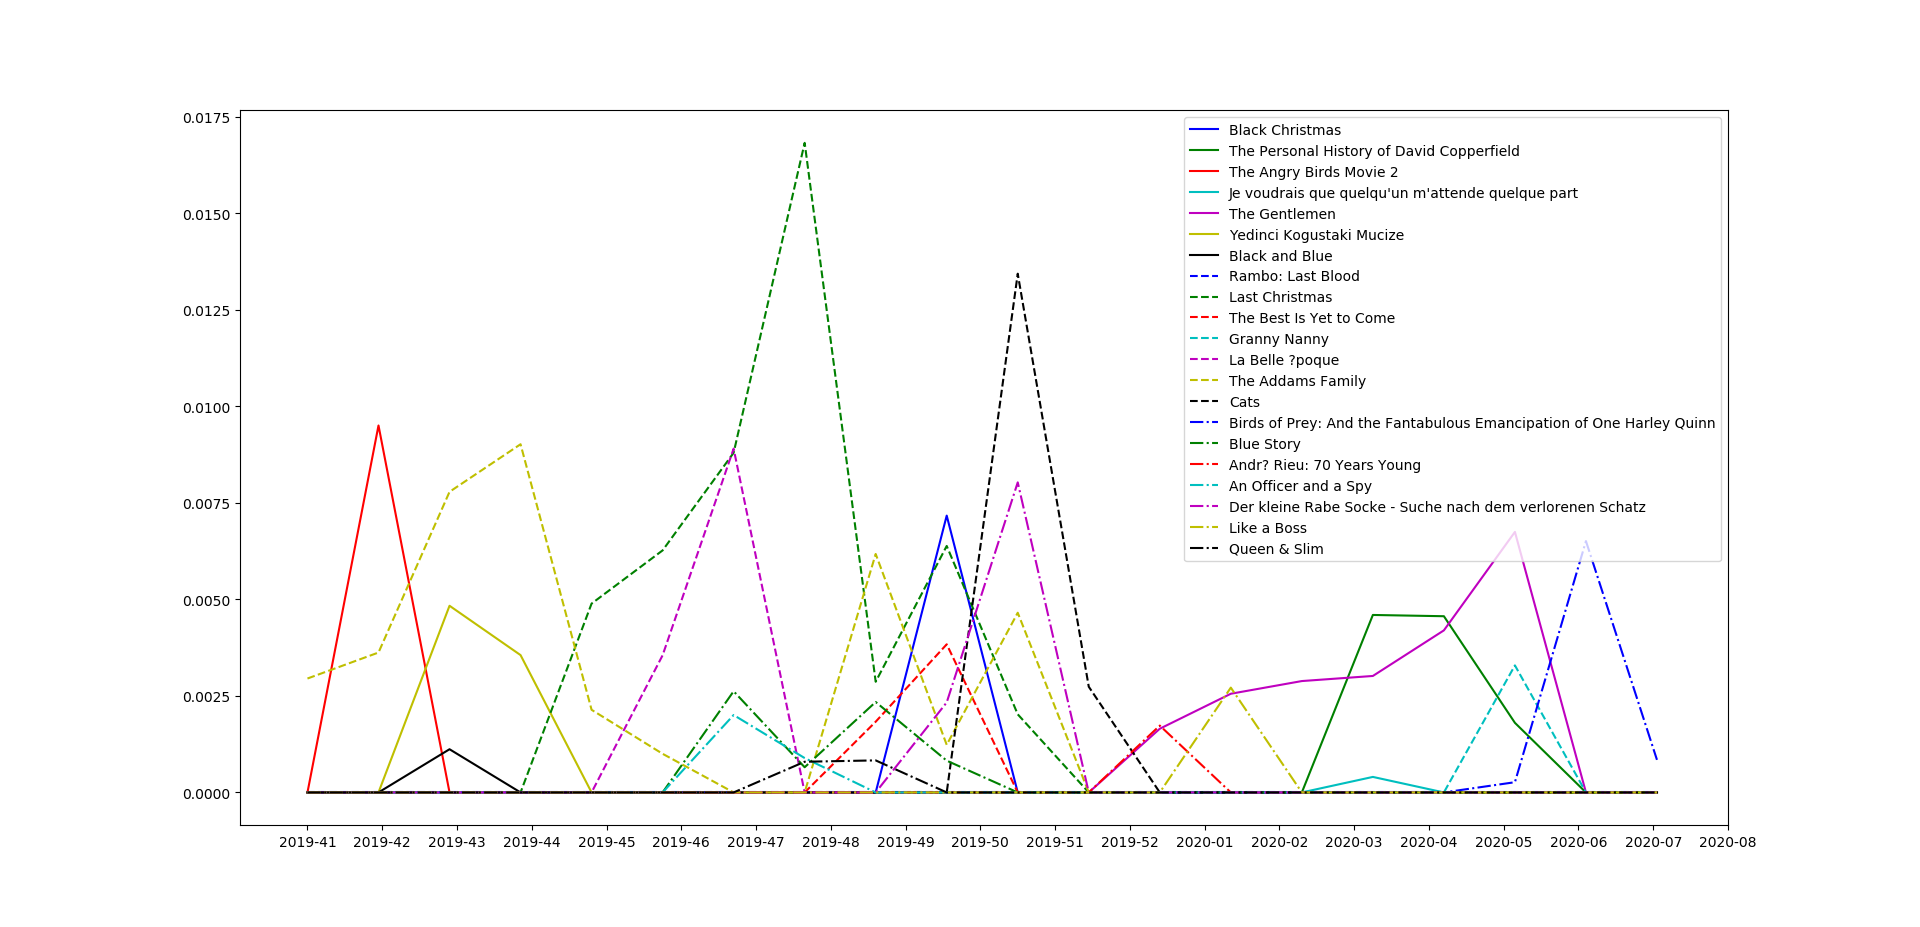
\includegraphics[width=\textwidth]{top5_box_office_usukfrde_results10000itev3_part1.png}
    \label{fig:resdyn1}
  \end{subfigure}
  \begin{subfigure}[b]{0.6\textwidth}
    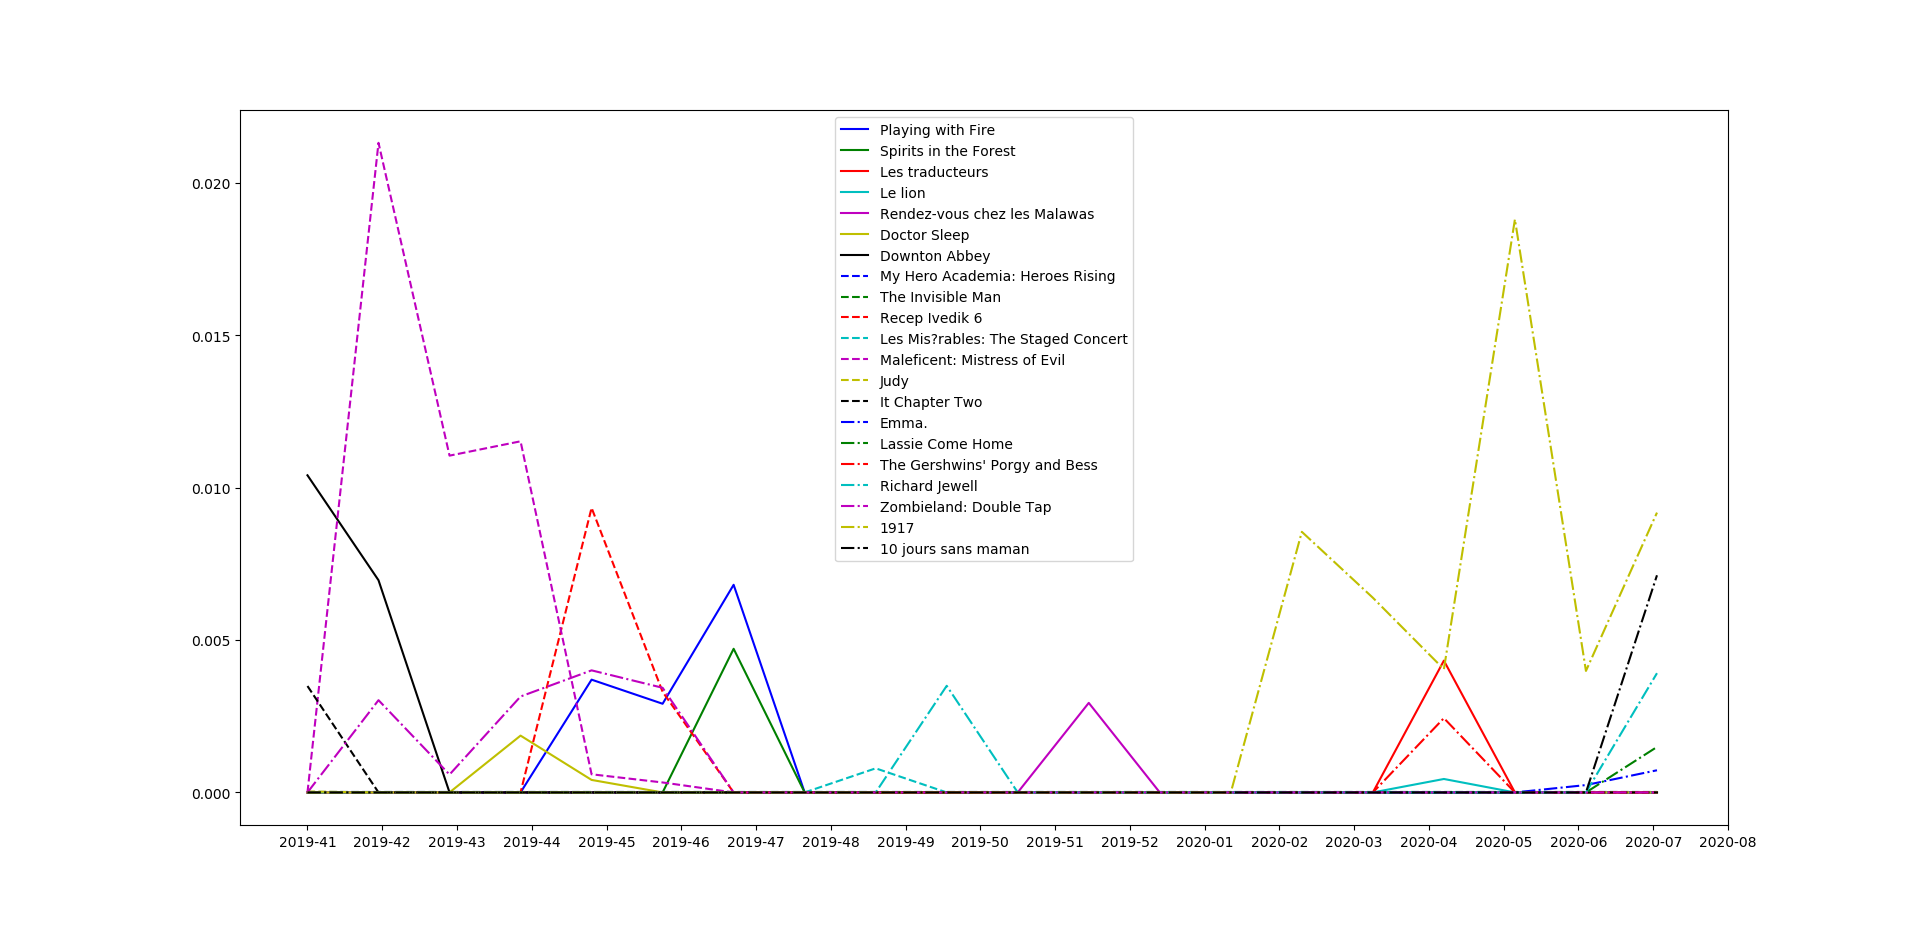
\includegraphics[width=\textwidth]{top5_box_office_usukfrde_results10000itev3_part2.png}
    \label{fig:resdyn2}
  \end{subfigure}
  \begin{subfigure}[b]{0.6\textwidth}
    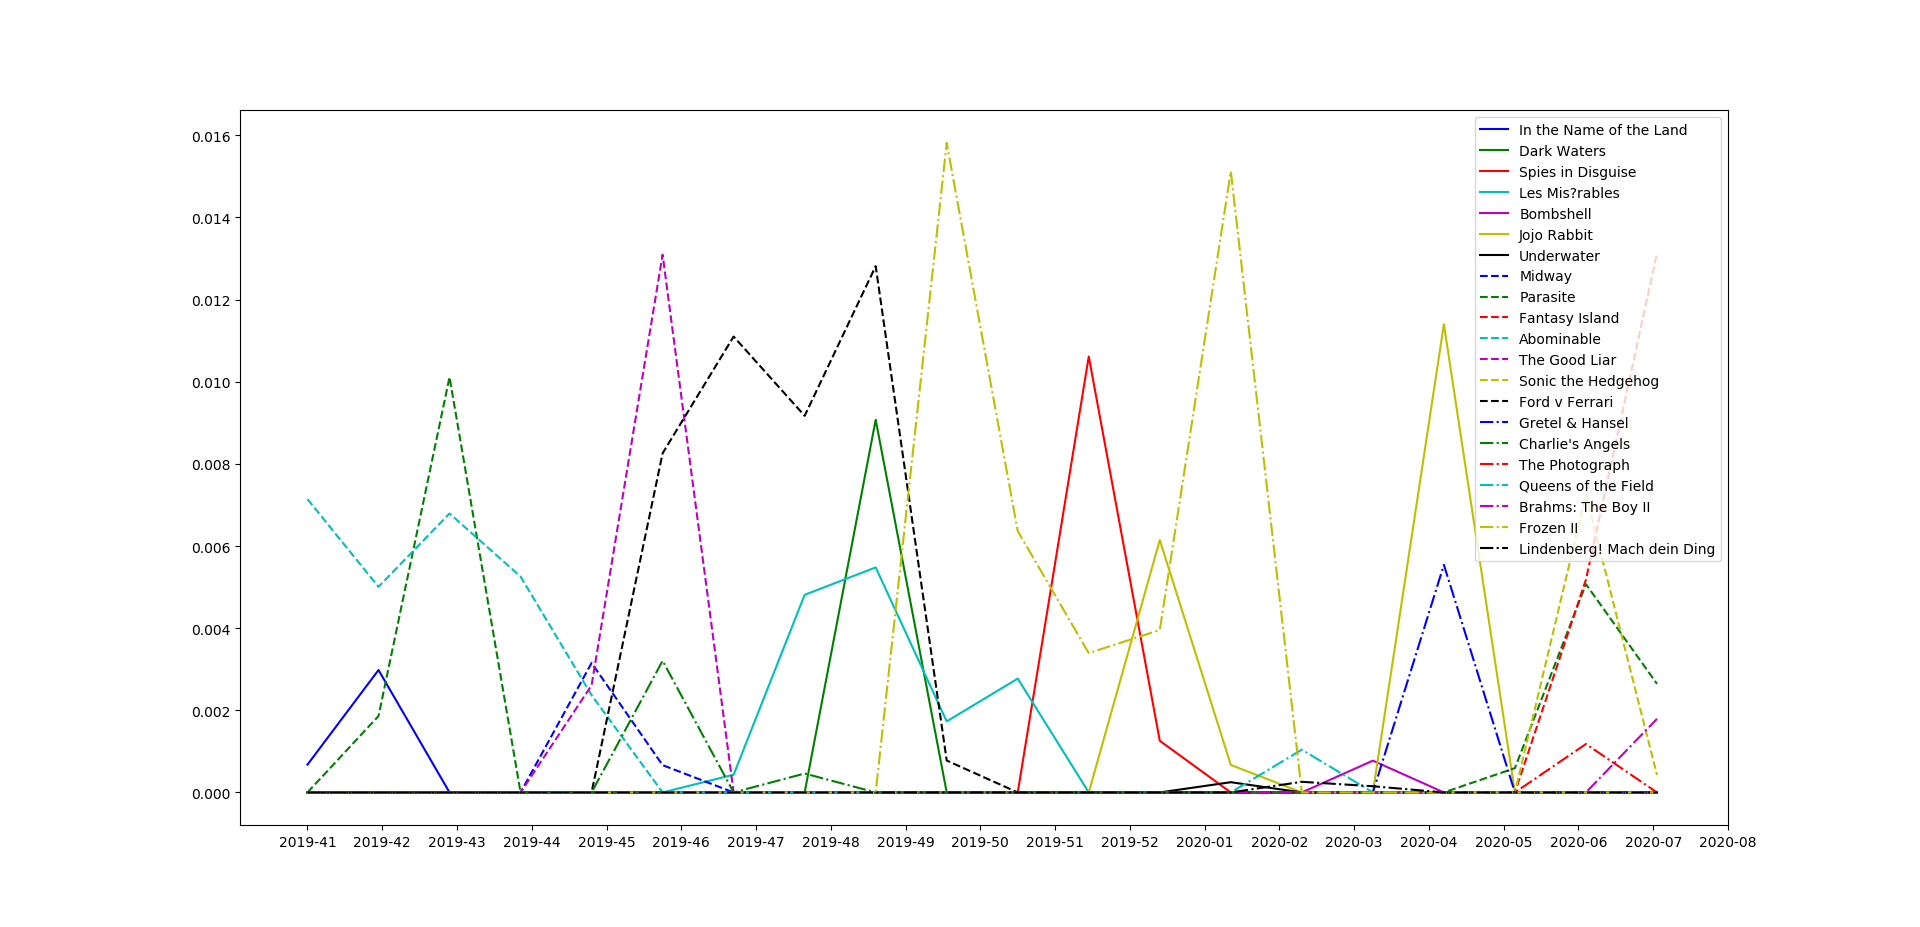
\includegraphics[width=\textwidth]{top5_box_office_usukfrde_results10000itev3_part3.png}
    \label{fig:resdyn3}
  \end{subfigure}
  \begin{subfigure}[b]{0.6\textwidth}
    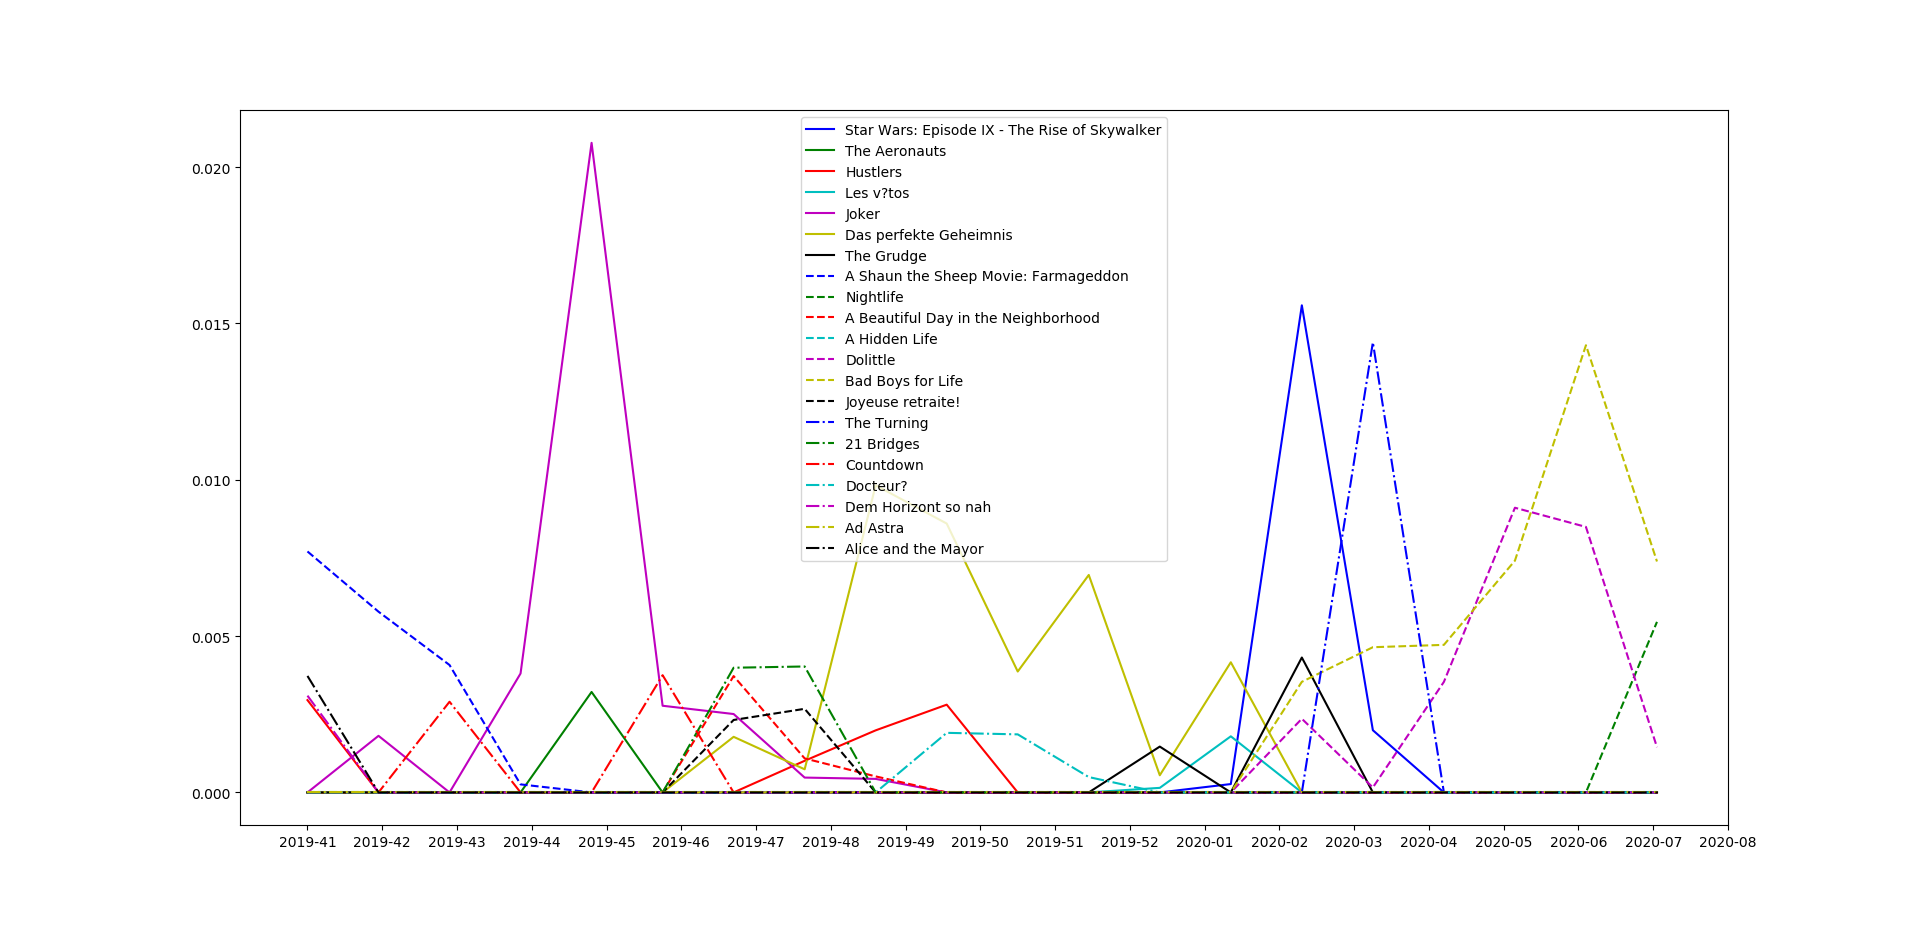
\includegraphics[width=\textwidth]{top5_box_office_usukfrde_results10000itev3_part4.png}
    \label{fig:resdyn4}
  \end{subfigure}
  \begin{subfigure}[b]{0.6\textwidth}
    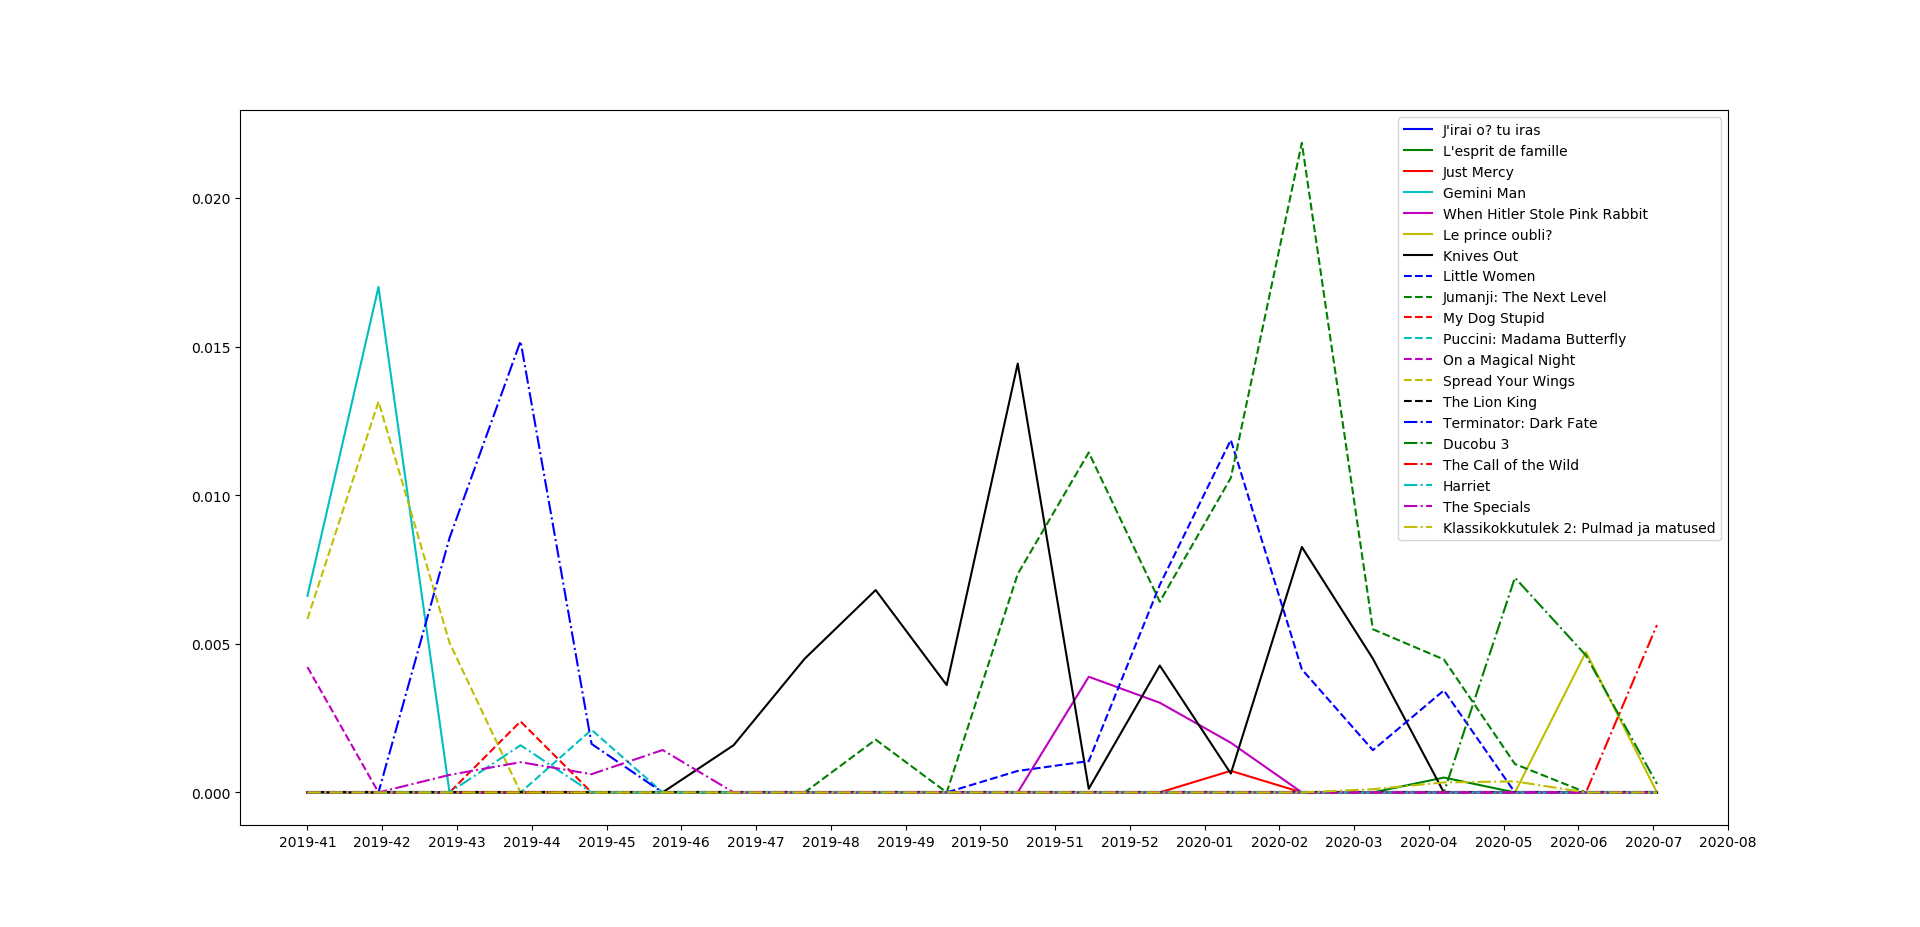
\includegraphics[width=\textwidth]{top5_box_office_usukfrde_results10000itev3_part5.png}
    \label{fig:resdyn5}
  \end{subfigure}
  \begin{subfigure}[b]{0.6\textwidth}
    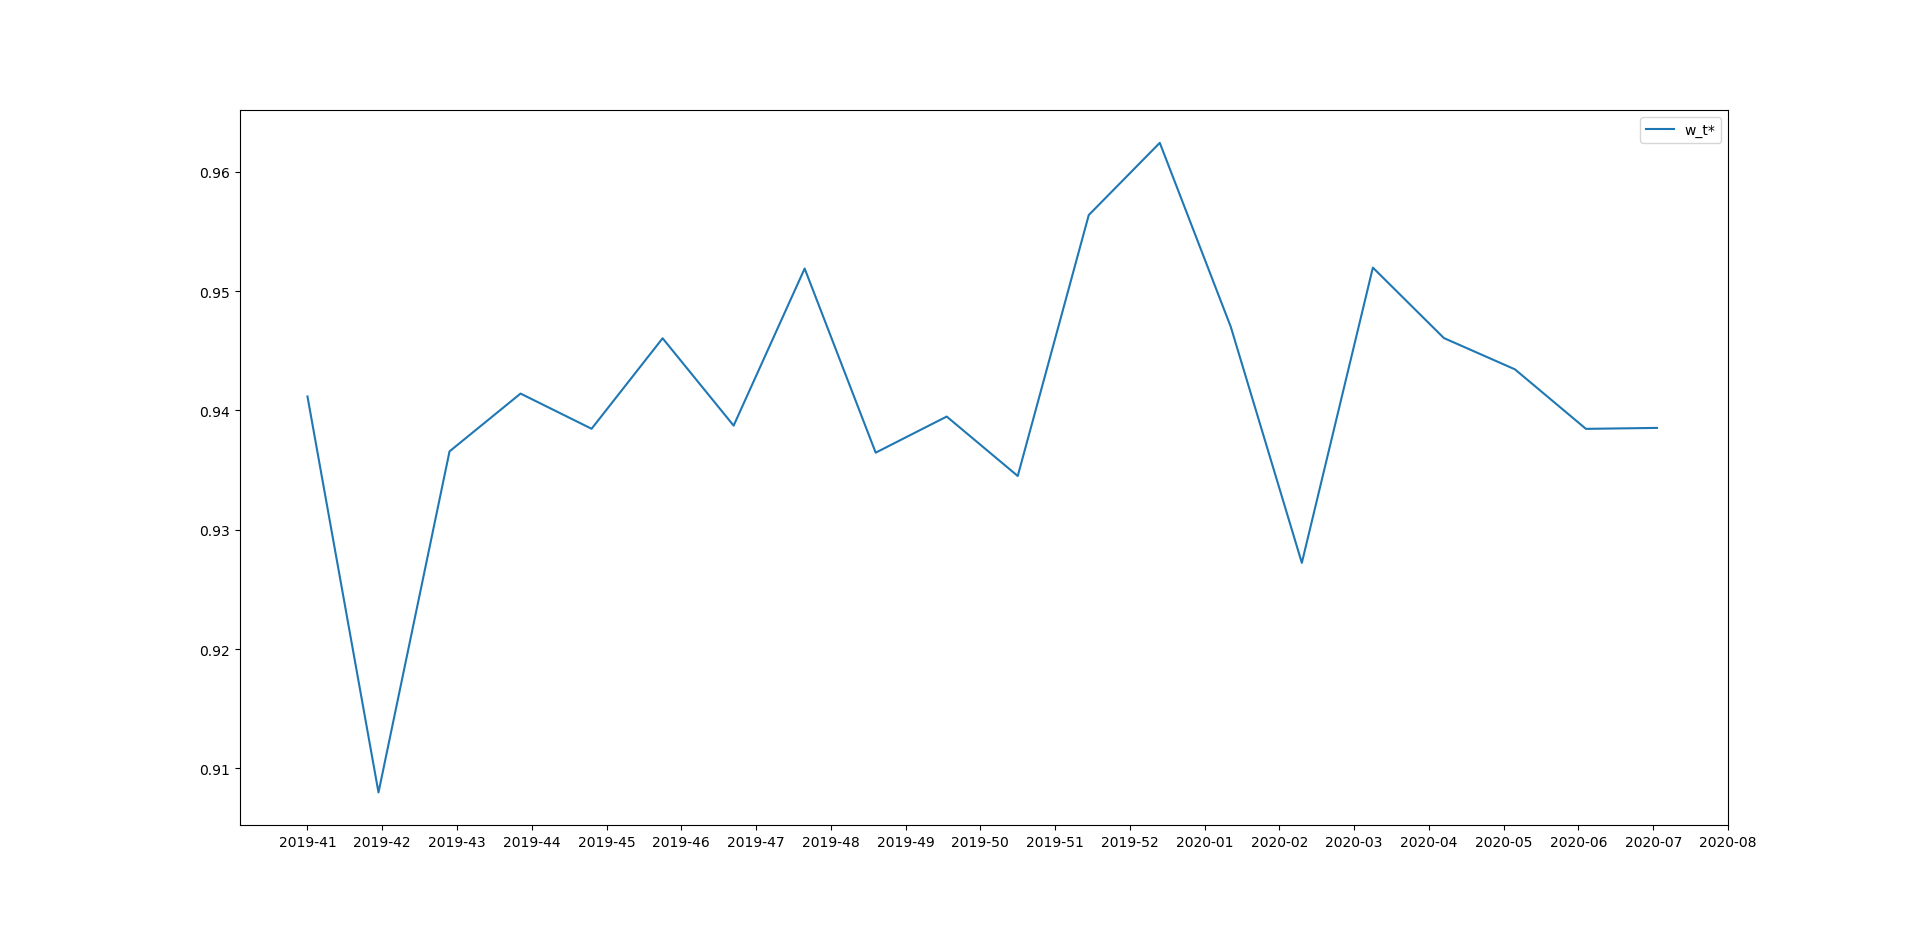
\includegraphics[width=\textwidth]{top5_box_office_usukfrde_results10000itev3_part6.png}
    \label{fig:resdyn6}
  \end{subfigure}
\caption{Evolution of the mean of samples of $w_{t,k}$ and $w_{t*}$}
\end{figure}

It looks like that the weights $w_{t*}$ seem to be over-estimated again -- even if we expected large $w_{t*}$ : if we pick any random country, it is likely that national movies are in the top-5 more successful movies only in this country. Maybe if we used more lists of rankings the results would be more accurate.



\bibliographystyle{plain}
\bibliography{bibli}


\end{document}
